% ============================================================
\chapter{Arbres de D\'ecision}
\label{ch:arbres}
\index{arbre de d\'ecision}
% ============================================================

\section{Principe g\'en\'eral}
\label{sec:arbres-principe}

Un \textbf{arbre de d\'ecision}\index{arbre de d\'ecision} est un mod\`ele
pr\'edictif qui partitionne r\'ecursivement l'espace des features par des
tests binaires sur les attributs, formant une structure arborescente.

\begin{definition}[Arbre de d\'ecision]
Un arbre de d\'ecision est un graphe acyclique orient\'e $T = (V, E)$ o\`u~:
\begin{itemize}
  \item Chaque n\oe{}ud interne $v \in V$ est associ\'e \`a un test
    $x_j \leq s$ (attribut $j$, seuil $s$).
  \item Chaque feuille $\ell$ contient une pr\'ediction~:
    la classe majoritaire (classification) ou la moyenne des $y_i$
    (r\'egression).
  \item Chaque ar\^ete repr\'esente le r\'esultat d'un test (vrai/faux).
\end{itemize}
\end{definition}

\begin{center}
\begin{tikzpicture}[
  node distance=1.2cm and 1.5cm,
  decision/.style={rectangle, draw, rounded corners, fill=blue!10,
    minimum width=2.5cm, minimum height=0.7cm, align=center,
    font=\small},
  leaf/.style={rectangle, draw, rounded corners, fill=green!15,
    minimum width=1.5cm, minimum height=0.6cm, align=center,
    font=\small\bfseries},
  edge label/.style={font=\scriptsize, midway}
]
  \node[decision] (r) {$x_1 \leq 5.5$~?};
  \node[decision, below left=of r] (l1) {$x_2 \leq 2.8$~?};
  \node[leaf, below right=of r] (f1) {Classe B};
  \node[leaf, below left=of l1] (f2) {Classe A};
  \node[leaf, below right=of l1] (f3) {Classe B};

  \draw[-{Stealth}] (r) -- node[edge label, left] {Oui} (l1);
  \draw[-{Stealth}] (r) -- node[edge label, right] {Non} (f1);
  \draw[-{Stealth}] (l1) -- node[edge label, left] {Oui} (f2);
  \draw[-{Stealth}] (l1) -- node[edge label, right] {Non} (f3);
\end{tikzpicture}
\end{center}

\section{Crit\`eres de s\'eparation}
\label{sec:criteres}
\index{crit\`ere de s\'eparation}

Soit un n\oe{}ud contenant un ensemble $S$ de $|S|$ exemples. On note $p_k$ la
proportion d'exemples de classe $k$ dans $S$~:
$p_k = \frac{|\{i \in S : y_i = k\}|}{|S|}$.

\subsection{Entropie de Shannon et gain d'information}
\index{entropie}

\begin{definition}[Entropie]
L'\textbf{entropie} de Shannon d'un n\oe{}ud $S$ est~:
\begin{equation}
  H(S) = -\sum_{k=1}^K p_k \log_2 p_k
  \label{eq:entropy}
\end{equation}
avec la convention $0 \log_2 0 = 0$. $H(S) = 0$ si le n\oe{}ud est pur
(une seule classe), $H(S) = \log_2 K$ si les classes sont \'equiprobables.
\end{definition}

\begin{definition}[Gain d'information]
\index{gain d'information}
Le \textbf{gain d'information} associ\'e \`a une s\'eparation de $S$ en
$S_L$ (gauche) et $S_R$ (droite) est~:
\begin{equation}
  \text{IG}(S, S_L, S_R) = H(S) - \frac{|S_L|}{|S|} H(S_L)
  - \frac{|S_R|}{|S|} H(S_R)
  \label{eq:info-gain}
\end{equation}
L'algorithme ID3 choisit la s\'eparation maximisant le gain d'information.
\end{definition}

\begin{proposition}[Positivit\'e du gain d'information]
Le gain d'information est toujours positif ou nul~:
$\text{IG}(S, S_L, S_R) \geq 0$, avec \'egalit\'e si et seulement si
$p_k(S_L) = p_k(S_R) = p_k(S)$ pour tout $k$.
\end{proposition}

\begin{proof}
C'est une cons\'equence directe de la concavit\'e de l'entropie. En effet,
l'entropie conditionnelle pond\'er\'ee est~:
\[
  H_{\text{cond}} = \frac{|S_L|}{|S|} H(S_L) + \frac{|S_R|}{|S|} H(S_R)
\]
Par concavit\'e de $H$ (comme fonction de la distribution)~:
$H_{\text{cond}} \leq H(S)$, d'o\`u $\text{IG} \geq 0$.
\end{proof}

\subsection{Impuret\'e de Gini}
\index{Gini}

\begin{definition}[Impuret\'e de Gini]
L'\textbf{impuret\'e de Gini} d'un n\oe{}ud $S$ est~:
\begin{equation}
  G(S) = 1 - \sum_{k=1}^K p_k^2 = \sum_{k=1}^K p_k(1 - p_k)
  \label{eq:gini}
\end{equation}
$G(S) = 0$ si le n\oe{}ud est pur. L'algorithme CART utilise ce crit\`ere
par d\'efaut.
\end{definition}

\begin{exemple}[Comparaison des crit\`eres]
Pour un probl\`eme binaire avec $p_1 = p$~:
\begin{align}
  H(S) &= -p\log_2 p - (1-p)\log_2(1-p) \\
  G(S) &= 2p(1-p)
\end{align}
Les deux crit\`eres atteignent leur maximum en $p = 0.5$ et leur minimum en
$p \in \{0, 1\}$. L'entropie est l\'eg\`erement plus sensible aux
distributions d\'es\'equilibr\'ees.
\end{exemple}

\begin{formules}[title=\textbf{R\'ecapitulatif des crit\`eres}]
\begin{center}
\begin{tabular}{lcc}
\toprule
\textbf{Crit\`ere} & \textbf{Formule} & \textbf{Utilis\'e par} \\
\midrule
Entropie & $-\sum_k p_k \log_2 p_k$ & ID3, C4.5 \\
Gini & $1 - \sum_k p_k^2$ & CART \\
Erreur de classification & $1 - \max_k p_k$ & (rarement) \\
\bottomrule
\end{tabular}
\end{center}
\end{formules}

\section{Algorithme CART}
\label{sec:cart}
\index{CART}

\begin{algorithme}[title=\textbf{Construction d'un arbre CART}]
\textbf{Entr\'ee}~: ensemble d'entra\^inement $S$, crit\`ere $Q$ (Gini ou
entropie).

\begin{enumerate}
  \item Si $S$ est pur ou un crit\`ere d'arr\^et est atteint, cr\'eer une
    feuille avec la pr\'ediction majoritaire.
  \item Sinon, pour chaque attribut $j$ et chaque seuil $s$~:
    \begin{enumerate}
      \item Partitionner $S$ en $S_L = \{i : x_{ij} \leq s\}$ et
        $S_R = \{i : x_{ij} > s\}$.
      \item Calculer la r\'eduction d'impuret\'e~:
        $\Delta Q = Q(S) - \frac{|S_L|}{|S|}Q(S_L) - \frac{|S_R|}{|S|}Q(S_R)$.
    \end{enumerate}
  \item Choisir $(j^*, s^*)$ maximisant $\Delta Q$.
  \item Cr\'eer un n\oe{}ud avec le test $x_{j^*} \leq s^*$.
  \item Appliquer r\'ecursivement sur $S_L$ et $S_R$.
\end{enumerate}
\textbf{Complexit\'e}~: $O(n \cdot d \cdot n \log n)$ par niveau (tri des
attributs), $O(n \cdot d \cdot n \log^2 n)$ au total.
\end{algorithme}

\section{Arbres de r\'egression}
\label{sec:regression-trees}
\index{arbre de d\'ecision!r\'egression}

Pour la r\'egression ($y_i \in \R$), on remplace l'impuret\'e par la variance
(ou l'erreur quadratique moyenne).

\begin{definition}[Crit\`ere de s\'eparation pour la r\'egression]
La r\'eduction de variance pour une partition $(S_L, S_R)$ est~:
\begin{equation}
  \Delta \text{Var} = \Var(S) - \frac{|S_L|}{|S|}\Var(S_L)
  - \frac{|S_R|}{|S|}\Var(S_R)
\end{equation}
o\`u $\Var(S) = \frac{1}{|S|}\sum_{i \in S}(y_i - \bar{y}_S)^2$ et
$\bar{y}_S = \frac{1}{|S|}\sum_{i \in S} y_i$.
\end{definition}

Chaque feuille $R_m$ pr\'edit la moyenne~:
\begin{equation}
  \hat{f}(\bm{x}) = \sum_{m=1}^M \bar{y}_{R_m} \cdot \ind[\bm{x} \in R_m]
\end{equation}

\section{\'Elagage}
\label{sec:pruning}
\index{\'elagage}

Un arbre complet (non \'elagu\'e) a tendance \`a surapprendre. L'\'elagage
(\emph{pruning}) r\'eduit la complexit\'e pour am\'eliorer la
g\'en\'eralisation.

\subsection{Pr\'e-\'elagage}
\index{\'elagage!pr\'e-\'elagage}

On impose des crit\`eres d'arr\^et \emph{avant} la construction~:
\begin{itemize}
  \item \texttt{max\_depth}~: profondeur maximale de l'arbre.
  \item \texttt{min\_samples\_split}~: nombre minimal d'exemples pour
    autoriser une s\'eparation.
  \item \texttt{min\_samples\_leaf}~: nombre minimal d'exemples dans chaque
    feuille.
  \item \texttt{max\_leaf\_nodes}~: nombre maximal de feuilles.
\end{itemize}

\subsection{Post-\'elagage par co\^ut-complexit\'e}
\index{\'elagage!co\^ut-complexit\'e}

\begin{definition}[Co\^ut-complexit\'e]
Pour un arbre $T$, on d\'efinit le crit\`ere de co\^ut-complexit\'e~:
\begin{equation}
  R_\alpha(T) = R(T) + \alpha \cdot |T|
  \label{eq:cost-complexity}
\end{equation}
o\`u $R(T) = \sum_{m=1}^{|T|} \frac{|R_m|}{n} \cdot Q(R_m)$ est l'erreur de
r\'esubstitution, $|T|$ le nombre de feuilles, et $\alpha \geq 0$ le
param\`etre de complexit\'e.
\end{definition}

\begin{theoreme}[\'Elagage optimal]
Pour chaque $\alpha$, il existe un unique plus petit sous-arbre
$T_\alpha \subseteq T_{\max}$ minimisant $R_\alpha(T)$. De plus, si
$\alpha_1 < \alpha_2$, alors $T_{\alpha_2} \subseteq T_{\alpha_1}$.
\end{theoreme}

L'algorithme proc\`ede ainsi~:
\begin{enumerate}
  \item Construire l'arbre maximal $T_{\max}$.
  \item Pour chaque n\oe{}ud interne $t$, calculer
    $\alpha_{\text{eff}}(t) = \frac{R(t) - R(T_t)}{|T_t| - 1}$ o\`u $T_t$
    est le sous-arbre enracin\'e en $t$.
  \item \'Elaguer le n\oe{}ud avec le plus petit $\alpha_{\text{eff}}$
    (remplacer le sous-arbre par une feuille).
  \item R\'ep\'eter jusqu'\`a obtenir la racine seule. Cela produit une
    s\'equence d'arbres $T_{\max} \supset T_1 \supset \cdots \supset T_0$.
  \item Choisir le meilleur $\alpha$ par validation crois\'ee.
\end{enumerate}

\begin{center}
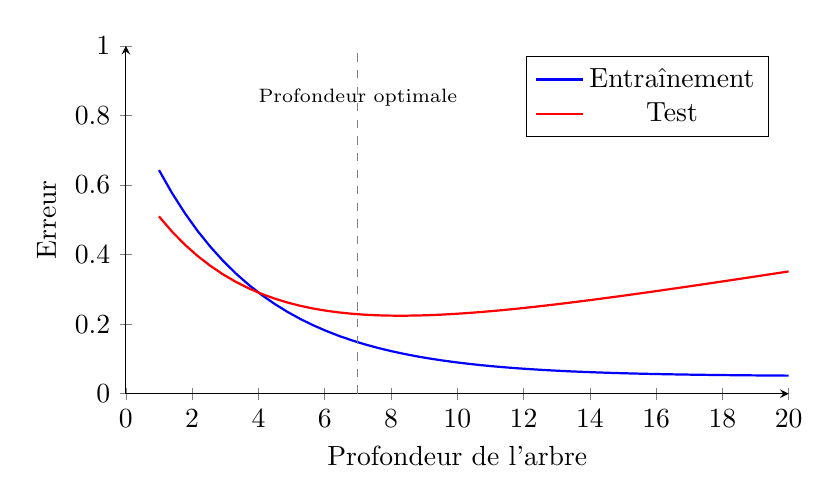
\begin{tikzpicture}
  \begin{axis}[
    width=10cm, height=6cm,
    xlabel={Profondeur de l'arbre},
    ylabel={Erreur},
    xmin=0, xmax=20, ymin=0, ymax=1,
    legend pos=north east,
    axis lines=left,
  ]
    \addplot[thick, blue, domain=1:20, samples=50]
      {0.05 + 0.8*exp(-0.3*x)};
    \addlegendentry{Entra\^inement}
    \addplot[thick, red, domain=1:20, samples=50]
      {0.05 + 0.6*exp(-0.3*x) + 0.015*x};
    \addlegendentry{Test}
    \draw[dashed, gray] (axis cs:7,0) -- (axis cs:7,1);
    \node[font=\scriptsize] at (axis cs:7,0.85) {Profondeur optimale};
  \end{axis}
\end{tikzpicture}
\end{center}

\section{Importance des variables}
\label{sec:feature-importance}
\index{importance des variables}

\begin{definition}[Importance MDI]
L'importance d'une variable $j$ est la r\'eduction totale d'impuret\'e
pond\'er\'ee apport\'ee par les s\'eparations sur $j$~:
\begin{equation}
  \text{Imp}(j) = \sum_{t : \text{split sur } j}
  \frac{|S_t|}{n} \Delta Q(t)
\end{equation}
normalis\'ee pour que $\sum_j \text{Imp}(j) = 1$.
\end{definition}

\section{Impl\'ementation avec scikit-learn}
\label{sec:arbres-sklearn}

\begin{codeblock}[title=\textbf{Arbre de d\'ecision sur le dataset Iris}]
\begin{minted}{python}
import numpy as np
import matplotlib.pyplot as plt
from sklearn.datasets import load_iris
from sklearn.tree import DecisionTreeClassifier, plot_tree
from sklearn.model_selection import (
    train_test_split, cross_val_score, GridSearchCV
)
from sklearn.metrics import accuracy_score

# Charger les donnees
X, y = load_iris(return_X_y=True)
feature_names = load_iris().feature_names
target_names = load_iris().target_names

X_train, X_test, y_train, y_test = train_test_split(
    X, y, test_size=0.3, random_state=42, stratify=y
)

# Arbre sans contrainte (surapprentissage)
tree_full = DecisionTreeClassifier(random_state=42)
tree_full.fit(X_train, y_train)
print("=== Arbre complet ===")
print(f"Accuracy train : {tree_full.score(X_train, y_train):.4f}")
print(f"Accuracy test  : {tree_full.score(X_test, y_test):.4f}")
print(f"Profondeur     : {tree_full.get_depth()}")
print(f"Nb feuilles    : {tree_full.get_n_leaves()}")

# Arbre elague (pre-elagage)
tree_pruned = DecisionTreeClassifier(
    max_depth=3, min_samples_leaf=5, random_state=42
)
tree_pruned.fit(X_train, y_train)
print("\n=== Arbre elague ===")
print(f"Accuracy train : {tree_pruned.score(X_train, y_train):.4f}")
print(f"Accuracy test  : {tree_pruned.score(X_test, y_test):.4f}")
print(f"Profondeur     : {tree_pruned.get_depth()}")
print(f"Nb feuilles    : {tree_pruned.get_n_leaves()}")
\end{minted}
\end{codeblock}

\begin{codeoutput}
\begin{verbatim}
=== Arbre complet ===
Accuracy train : 1.0000
Accuracy test  : 0.9556
Profondeur     : 5
Nb feuilles    : 9

=== Arbre elague ===
Accuracy train : 0.9714
Accuracy test  : 0.9556
Profondeur     : 3
Nb feuilles    : 5
\end{verbatim}
\end{codeoutput}

\begin{codeblock}[title=\textbf{Visualisation de l'arbre et importance des variables}]
\begin{minted}{python}
# Visualisation de l'arbre
fig, ax = plt.subplots(figsize=(14, 8))
plot_tree(tree_pruned, feature_names=feature_names,
          class_names=target_names, filled=True, rounded=True,
          fontsize=9, ax=ax)
plt.title("Arbre de decision (Iris, max_depth=3)")
plt.tight_layout()
plt.savefig("arbre_iris.pdf")

# Importance des variables
importances = tree_pruned.feature_importances_
indices = np.argsort(importances)[::-1]

fig, ax = plt.subplots(figsize=(8, 4))
ax.barh(range(len(importances)), importances[indices], color="steelblue")
ax.set_yticks(range(len(importances)))
ax.set_yticklabels([feature_names[i] for i in indices])
ax.set_xlabel("Importance (MDI)")
ax.set_title("Importance des variables")
plt.tight_layout()
plt.savefig("arbre_importance.pdf")

print("Importance des variables :")
for i in indices:
    print(f"  {feature_names[i]:25s} : {importances[i]:.4f}")
\end{minted}
\end{codeblock}

\begin{codeoutput}
\begin{verbatim}
Importance des variables :
  petal width (cm)          : 0.5815
  petal length (cm)         : 0.4040
  sepal length (cm)         : 0.0146
  sepal width (cm)          : 0.0000
\end{verbatim}
\end{codeoutput}

\begin{codeblock}[title=\textbf{Post-\'elagage par co\^ut-complexit\'e}]
\begin{minted}{python}
# Chemin de cout-complexite
path = tree_full.cost_complexity_pruning_path(X_train, y_train)
ccp_alphas = path.ccp_alphas[:-1]  # exclure le dernier (arbre trivial)

# Entrainer un arbre pour chaque alpha
trees = []
for alpha in ccp_alphas:
    t = DecisionTreeClassifier(ccp_alpha=alpha, random_state=42)
    t.fit(X_train, y_train)
    trees.append(t)

# Scores
train_scores = [t.score(X_train, y_train) for t in trees]
test_scores = [t.score(X_test, y_test) for t in trees]

fig, ax = plt.subplots(figsize=(8, 5))
ax.plot(ccp_alphas, train_scores, "o-", label="Train", markersize=3)
ax.plot(ccp_alphas, test_scores, "o-", label="Test", markersize=3)
ax.set_xlabel(r"$\alpha$ (cout-complexite)")
ax.set_ylabel("Accuracy")
ax.legend()
ax.set_title("Elagage par cout-complexite")
plt.tight_layout()
plt.savefig("arbre_ccp.pdf")

best_idx = np.argmax(test_scores)
print(f"Meilleur alpha : {ccp_alphas[best_idx]:.4f}")
print(f"Accuracy test  : {test_scores[best_idx]:.4f}")
\end{minted}
\end{codeblock}

\begin{codeoutput}
\begin{verbatim}
Meilleur alpha : 0.0148
Accuracy test  : 0.9778
\end{verbatim}
\end{codeoutput}

\section{Fronti\`ere de d\'ecision}
\label{sec:arbres-frontiere}

\begin{codeblock}[title=\textbf{Visualisation de la fronti\`ere de d\'ecision}]
\begin{minted}{python}
from sklearn.inspection import DecisionBoundaryDisplay

# Utiliser 2 features pour la visualisation
X2 = X[:, 2:4]  # petal length, petal width
X2_train, X2_test, y2_train, y2_test = train_test_split(
    X2, y, test_size=0.3, random_state=42, stratify=y
)

fig, axes = plt.subplots(1, 3, figsize=(15, 4))
for ax, depth in zip(axes, [1, 3, None]):
    tree = DecisionTreeClassifier(max_depth=depth, random_state=42)
    tree.fit(X2_train, y2_train)
    DecisionBoundaryDisplay.from_estimator(
        tree, X2_train, ax=ax, alpha=0.3, cmap=plt.cm.Set3
    )
    ax.scatter(X2_train[:, 0], X2_train[:, 1], c=y2_train,
               cmap=plt.cm.Set1, edgecolors="k", s=20)
    acc = tree.score(X2_test, y2_test)
    title = f"depth={depth}" if depth else "depth=infini"
    ax.set_title(f"{title} (acc={acc:.2f})")
    ax.set_xlabel("petal length")
    ax.set_ylabel("petal width")
plt.tight_layout()
plt.savefig("arbre_frontieres.pdf")
\end{minted}
\end{codeblock}

\section{Exercices}
\label{sec:exercises-ch6}

\begin{exercice}[Calcul d'entropie et de Gini --- Niveau 1]
Un n\oe{}ud contient 30 exemples~: 10 de classe A, 15 de classe B, 5 de
classe C.
\begin{enumerate}
  \item Calculer l'entropie $H$ et l'impuret\'e de Gini $G$ de ce n\oe{}ud.
  \item On propose la s\'eparation suivante~: $S_L$ contient $(8, 2, 0)$ et
    $S_R$ contient $(2, 13, 5)$. Calculer le gain d'information et la
    r\'eduction de Gini.
  \item Comparer avec la s\'eparation $S_L = (5, 7, 3)$, $S_R = (5, 8, 2)$.
    Quelle s\'eparation est pr\'ef\'erable et pourquoi~?
\end{enumerate}
\end{exercice}

\begin{exercice}[Construction manuelle d'un arbre --- Niveau 2]
Consid\'erons le jeu de donn\'ees suivant ($x_1, x_2 \in \R$, $y \in
\{0, 1\}$)~:
\begin{center}
\begin{tabular}{ccc}
\toprule
$x_1$ & $x_2$ & $y$ \\
\midrule
1 & 3 & 0 \\
2 & 1 & 0 \\
3 & 2 & 0 \\
5 & 4 & 1 \\
6 & 3 & 1 \\
7 & 5 & 1 \\
4 & 6 & 1 \\
4 & 1 & 0 \\
\bottomrule
\end{tabular}
\end{center}
\begin{enumerate}
  \item Construire un arbre CART (crit\`ere Gini) en d\'etaillant chaque
    \'etape~: \'enum\'erer tous les seuils candidats, calculer les impuret\'es,
    s\'electionner la meilleure s\'eparation.
  \item D\'eterminer la profondeur minimale n\'ecessaire pour classer
    correctement tous les exemples.
  \item V\'erifier votre r\'esultat avec \texttt{DecisionTreeClassifier}.
\end{enumerate}
\end{exercice}

\begin{exercice}[Analyse th\'eorique et pratique --- Niveau 3]
\begin{enumerate}
  \item D\'emontrer que pour un probl\`eme binaire, l'impuret\'e de Gini et
    l'entropie satisfont $G(p) \leq H(p) / \ln 2$ pour tout $p \in [0, 1]$.
    (\emph{Indication}~: utiliser $\ln x \leq x - 1$.)
  \item Montrer que l'erreur de classification $1 - \max_k p_k$ n'est pas un
    bon crit\`ere de s\'eparation en donnant un contre-exemple o\`u elle ne
    diff\'erencie pas deux partitions de qualit\'es diff\'erentes.
  \item Sur le dataset \texttt{wine} de scikit-learn, comparer
    syst\'ematiquement les crit\`eres Gini et entropie en termes d'accuracy
    (validation crois\'ee 10-fold), de profondeur et de nombre de feuilles,
    pour diff\'erentes valeurs de \texttt{max\_depth}.
  \item Impl\'ementer un arbre de d\'ecision CART complet \`a partir de z\'ero
    (sans scikit-learn) pour la classification binaire. Comparer avec
    \texttt{DecisionTreeClassifier} sur le dataset \texttt{make\_moons}.
\end{enumerate}
\end{exercice}
